\chapter{序論}
\label{chap:introduction}

本章では、本研究の背景と目的、及び本論文の構成について述べる。

\newpage

\section{背景}
パーソナルコンピュータの普及に伴いアプリケーションの数はますます増加しており、個人が使うアプリケーションの数も自ずと増えてきた。数多くのアプリケーションの中から目的のアプリケーションを起動する方法としてアプリケーションランチャーは非常に有用であり、現在ではオペレーティングシステムにも標準で搭載されるようになった。またサードパーティ製として多くのソフトウェアが開発/公開されており、その形式も様々である。
その中でも、ホットキーを利用したアプリケーションランチャーは、特定のキーの入力のみでアプリケーションを起動することができる強力な機能である。しかし未習熟者には使いこなすのが難しく、あまり普及していないのが現状である。

\subsection{形式と比較}
現在使用されているアプリケーションランチャーの形式を大きく4つに分類し、それぞれの利点/欠点を比較していく。なお分類についてはWikipediaのランチャーについてのページ\footnote{https://ja.wikipedia.org/wiki/ランチャー\#コンピュータ}を参考にした。

\subsubsection{パレット型}

画面上の一部に固定されたパレット型のエリアにアプリケーションを登録し、マウスによるクリックで起動する形式のランチャー。macOSにおけるDock(図\ref{fig:dock})がこれにあたる。デスクトップに常駐しているため誰でも簡単に使用することができる。しかしそのエリアは有限であり、多くのアプリケーションを登録するためには、ボタンの数を増やしたりそれぞれを小さく表示したりする必要がある。その数が増えれば増えるほど操作ステップが増えるため、数個から数十個のよく使うアプリケーションを登録して使用するのが推奨される。

\begin{figure}[h]
    \begin{center}
       \fbox{
\includegraphics[width=100mm]{images/dock}}
    \end{center}
    \caption{Dock}
    \label{fig:dock}
\end{figure}

\subsubsection{メニュー型}

上述したDock等にメニューを設け、マウスを使用して登録したアプリケーションを起動できるようにする形式のランチャー。ホットキーと組み合わせて使用されるものもある。複数のアプリケーションを一つにまとめることで場所を節約できるだけでなく、階層化によって自分の使いやすいように整理することもできる。しかし、項目や階層が増えれば目的のアプリケーションに辿り着くまでの操作ステップは増えることになるため、稀に使用するアプリケーションを整理するために使うのが一般的である。

\newpage

\begin{figure}[h]
    \begin{center}
       \fbox{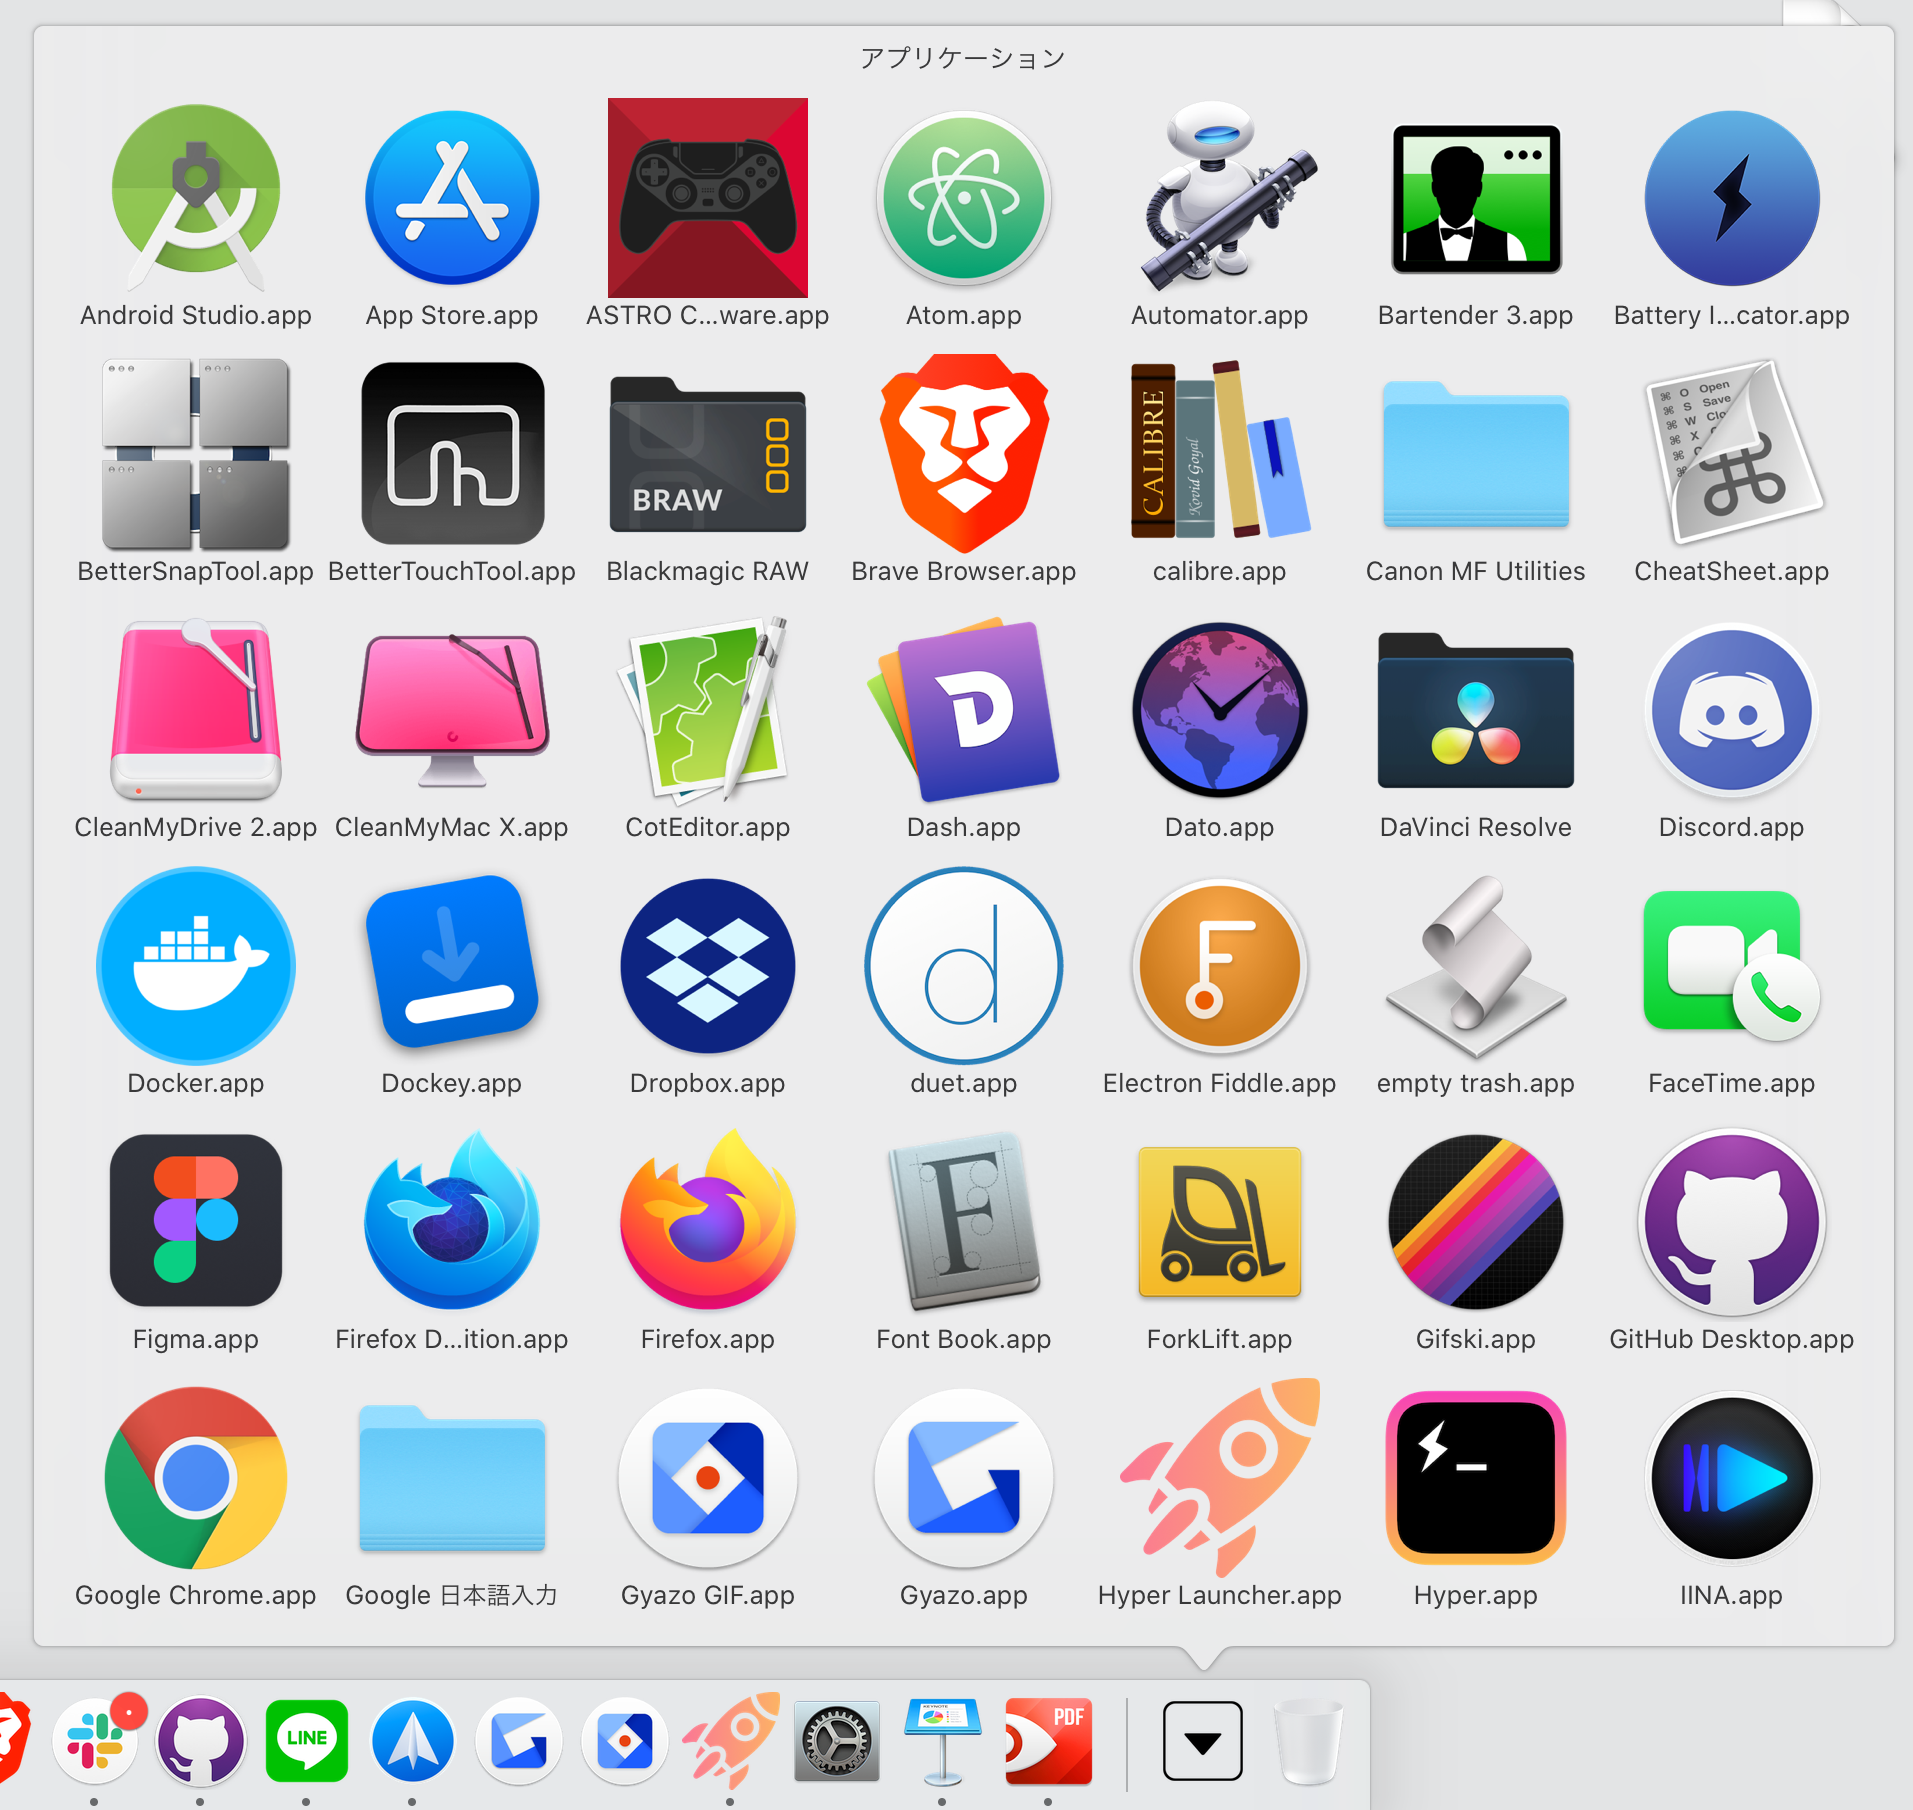
\includegraphics[width=100mm]{images/menu}}
    \end{center}
    \caption{Dock内のメニュー}
    \label{fig:menu}
\end{figure}

\subsubsection{検索型}

アプリケーションの名前を入力することで対象のアプリケーションを検索し起動する形式のランチャー。macOSにおけるSpotlightがこれにあたる。検索メニューは使用するときのみ表示されるため使用していない時は場所をとらないことに加え、キーボードのみで操作で完結するようになっている。もちろんマウスと組み合わせて使用することもできる。また大抵の場合インクリメンタルサーチが導入されているため、アプリケーションの名前を完全に覚えていなくても起動することができる。しかし、汎用性が高い反面、毎回一定のキーボード入力が必要となってしまうため、素早く複数のアプリケーションを切り替えるような操作には不向きである。

\begin{figure}[h]
    \begin{center}
       \fbox{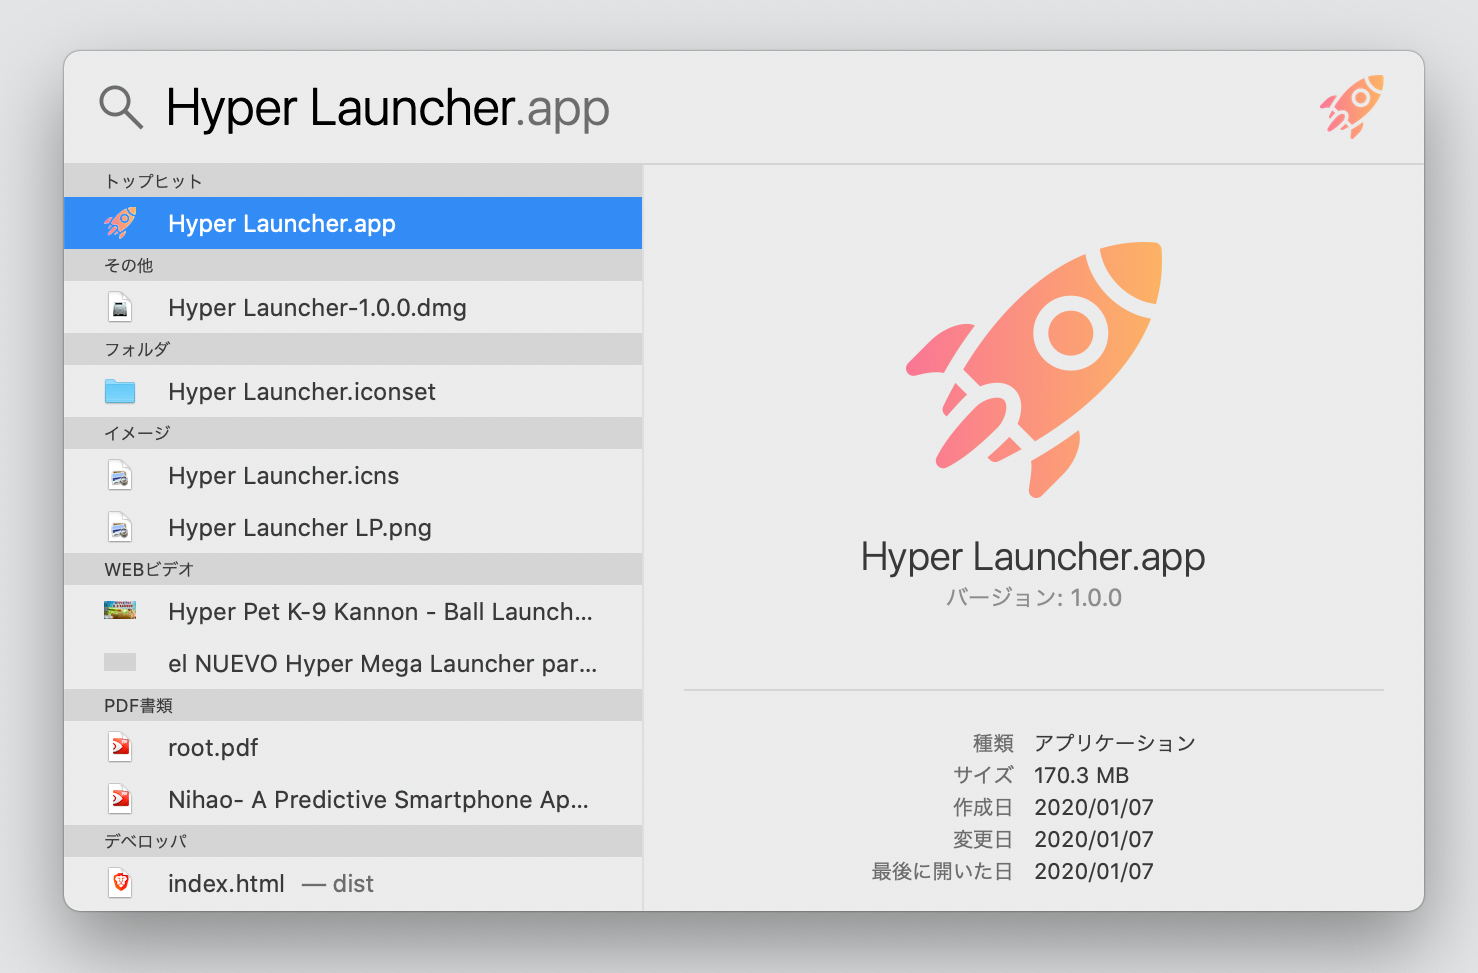
\includegraphics[width=100mm]{images/spotlight}}
    \end{center}
    \caption{Spotlight}
    \label{fig:spotlight}
\end{figure}

\subsubsection{ホットキー型}

単一のキーもしくは複数のキーの組み合わせを入力するだけで、登録したアプリケーションを起動できる形式のランチャー。他の形式のものとは違い、オペレーティングシステムに標準で搭載されていないことが多く、サードパーティ製ソフトウェアを自分で探す必要がある。普段は画面上に情報を表示する必要がないため場所をとらないが、その分どのホットキーにどのアプリケーションを登録したのか覚えておかなければならない。また、その設定画面のUIも使いやすいとは言えず、未習熟者には使いにくい形式だとされているのも事実である。
一発で特定のアプリケーションを起動できるというのはとても強力な機能ではあるが、あまり普及していないのはこれらの問題が原因だと考えられる。

\subsection{既存のアプリケーション}

先述した通り、ホットキーを利用したアプリケーションランチャーは標準で搭載されておらず、使用者自ら使いやすいものを探す必要がある。しかしその種類は豊富とは言えず、突出した特徴があるわけでもない。例として筆者が日常的に使用してきた2つのアプリケーションランチャーを示す。

\subsubsection{PMenu}

PMenu\footnote{https://danadesign.ltd/}(図\ref{fig:pmenu})はホットキーとメニューを利用したランチャーで、アプリケーションだけでなく様々なファイルをコマンドで操作することができる。使い勝手はいたって普通で可もなく不可もなくと言ったところである。自分の好きなホットキーを割り当てられるのは便利であるが、キーを登録するためのステップが多くとても煩雑で、こまめに切り替えるような使い方には向いていない。コンテキストメニューを利用することが主な方法とされているため、ホットキーに関しては最低限の機能が実装されているだけと言える。

\begin{figure}[h]
    \begin{center}
       \fbox{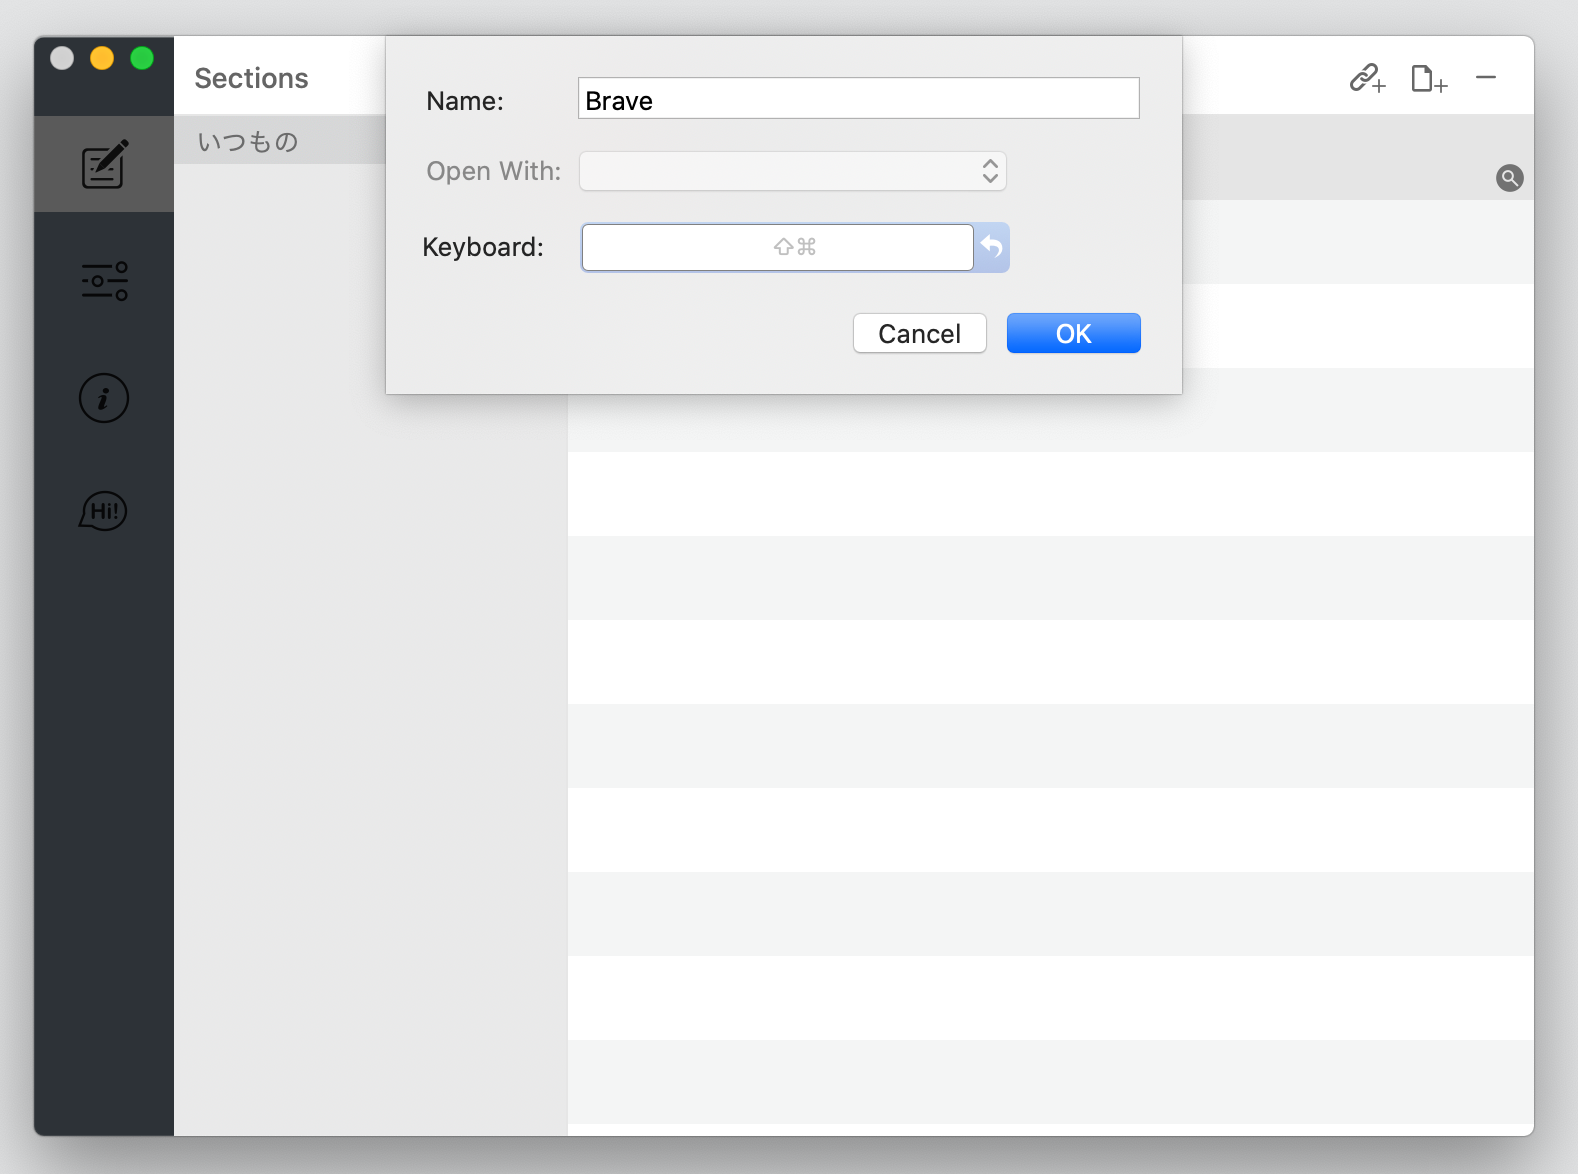
\includegraphics[width=100mm]{images/pmenu}}
    \end{center}
    \caption{PMenu}
    \label{fig:pmenu}
\end{figure}

\subsubsection{Snap}

Snap\footnote{https://apps.apple.com/jp/app/snap/id418073146}(図\ref{fig:snap})はホットキーを利用したランチャーで、macOSのDockを生かした機能が備わっている。SnapではDockに登録されたアプリケーションに左から順に数字を割り当てていき、その数字と設定したモディファイアキーとの組み合わせでアプリケーションを起動できるようになっている。これにより面倒な設定をすることなくホットキーの恩恵を授かることが可能となる。ただしDockのサイズは有限であり画面上に場所もとるため、多くのアプリケーションを登録するというのはあまり現実的ではない。ホットキーの設定も可能ではあるが、PMenuと同様操作ステップが多く使いやすいという印象は受けない。

\begin{figure}[h]
    \begin{center}
       \fbox{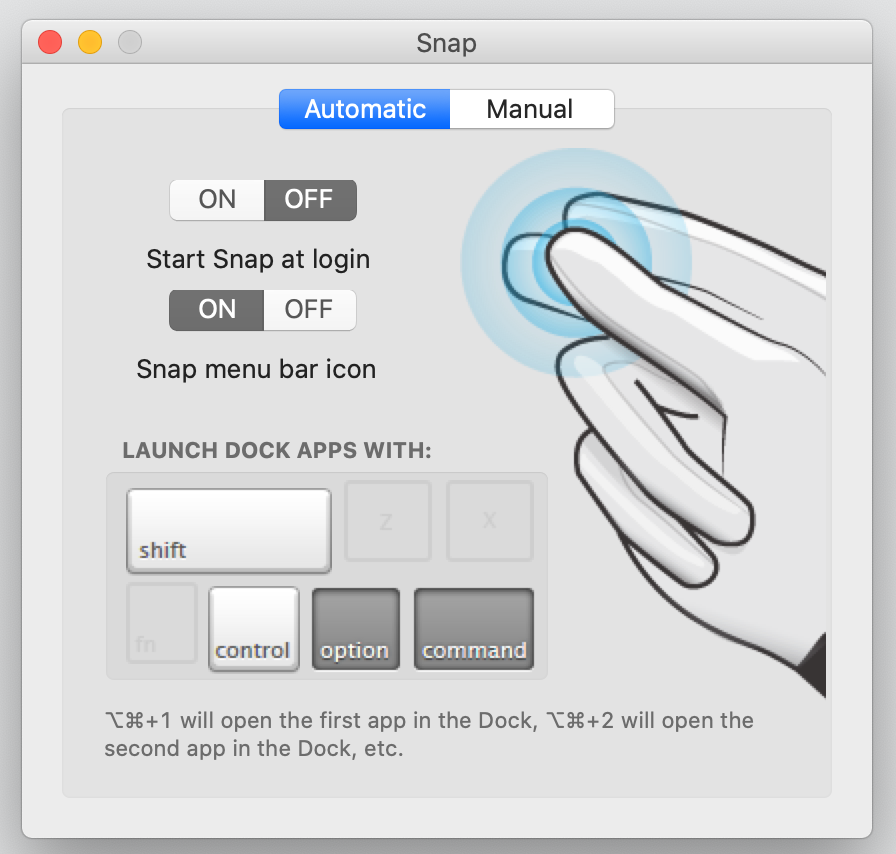
\includegraphics[width=100mm]{images/snap}}
    \end{center}
    \caption{Snap}
    \label{fig:snap}
\end{figure}

\subsection{運用例}
「macOSでディスプレイ1枚で作業する技術」\footnote{https://qiita.com/saboyutaka/items/d6cfd2a2b60f1a374d60}では、実際にホットキーを運用している例が紹介されている。本記事では、maOSの仮想デスクトップを10個に増やし、それぞれにアプリケーションとホットキーを割り当てることで、ランチャーと同等の機能を実現している。記事内では、ホットキーを覚えるのは大変だが、特定のキーを押すことで必ず指定されたアプリケーションが起動されるというのは安心感が得られるとされている。また、デスクトップ上でアプリケーションを探す手間も解消されている。
もちろん、他のホットキー型アプリケーションランチャーと同様の問題点はあるものの、その便利さがよく表れている例である。

\subsection{問題点}
ホットキー型のアプリケーションランチャーには、特定のアプリケーションをキーの入力のみで素早く起動できるという利点があるが、設定が煩雑であったり設定を覚える必要があったりするなど、使いこなせるようになるまでに大きな障壁がある。
また、その機能についても新しい手法が開発されることは少なく、機能及び利便性の両面でまだまだ改善の余地があると考えられる。

\section{本研究の目的}
既存のホットキー型アプリケーションランチャーにおける不便や機能の不足を解消し、より強力でより多くの人に使いやすいシステムを開発することが本研究の目的である。

\section{本論文の構成}

第1章では、本研究における背景と問題意識、目的について述べた。

第2章では、第1章で述べた問題意識を踏まえ、新しいホットキー型アプリケーションランチャーシステムを提案する。

第3章ではシステムの実装に関して述べ、第4章では実際に運用して得られた評価について述べる。

第5章では関連研究を交えシステムの議論を行い、第6で本研究を総括する。